\section{Results}
\label{sec:results}

We first show how merge order changes segmentation (\secref{sec:intrinsics}).
We then show its effect on language modeling (\secref{sec:lm}) and the compression mechanism behind it (\secref{sec:mechanism}).
Next we show that the effect does not reach fine-tuned classification (\secref{sec:ft}).
We close with robustness checks (\secref{sec:robustness}) and hypothesis verdicts (\secref{sec:verdicts}).

\subsection{Merge order changes segmentation drastically}
\label{sec:intrinsics}

\begin{table}[t]
    \centering
    \caption{Tokenizer intrinsics on held-out general / biomedical text. ``Top-1k whole'' is the share of the 1,000 most frequent words encoded as a single token. ``Vocab used'' is the share of the 8,192 entries that occur in 5M encoded tokens. ``Agree'' is segmentation agreement with \freq on general text. The application-order tokenizers share \freq's vocabulary but use only 21--41\% of it. Best value per column in \textbf{bold}.}
    \label{tab:intrinsics}
    \resizebox{\textwidth}{!}{%
    \begin{tabular}{@{}lcccccccc@{}}
        \toprule
        & \multicolumn{2}{c}{\textbf{Bytes / token} $\uparrow$} & \multicolumn{2}{c}{\textbf{Top-1k whole} $\uparrow$} & \multicolumn{1}{c}{\textbf{R\'enyi eff.}} & \textbf{Vocab} & \textbf{Agree} & \textbf{LM train} \\
        \cmidrule(lr){2-3} \cmidrule(lr){4-5}
        \textbf{Tokenizer} & Gen. & Dom. & Gen. & Dom. & Gen. & \textbf{used} & \textbf{w/ \freq} & \textbf{tokens} \\
        \midrule
        \freq      & \textbf{3.87} & 4.11          & \textbf{0.89} & 0.92          & 0.52 & \textbf{0.99} & 1.00 & \textbf{51.0M} \\
        \domain    & 3.65          & \textbf{4.41} & 0.82          & \textbf{0.99} & 0.54 & \textbf{0.99} & 0.88 & 52.5M \\
        \midrule
        \randlearn & 1.82          & 1.78          & 0.09          & 0.10          & 0.34 & 0.91 & 0.25 & 110.0M \\
        \revlearn  & 1.03          & 1.03          & 0.03          & 0.06          & 0.32 & 0.50 & 0.05 & 194.6M \\
        \midrule
        \randorder & 2.34          & 2.24          & 0.28          & 0.25          & \textbf{0.55} & 0.41 & 0.57 & 86.4M \\
        \revorder  & 1.73          & 1.71          & 0.10          & 0.10          & 0.44 & 0.21 & 0.28 & 116.1M \\
        \bottomrule
    \end{tabular}}
\end{table}


\para{Reordering the same merges breaks long tokens.}
\Tabref{tab:intrinsics} shows that \randorder and \revorder, which have \freq's exact vocabulary, pack 40--55\% fewer bytes into each token than \freq on general text (2.34 and 1.73 \versus 3.87 bytes per token).
They also keep only 28\% and 10\% of the top-1k words whole, compared with 89\% for \freq.
The reason is that merges compete for the same bytes.
When a short merge is applied first, it consumes bytes that a longer, frequent merge needed, and the long merge can no longer fire.
The word ``\,hypertension'' illustrates this:

\begin{center}
\small
\begin{tabular}{@{}ll@{}}
    \toprule
    \textbf{Tokenizer} & \textbf{Segmentation of ``\,hypertension''} \\
    \midrule
    \freq      & \texttt{\textvisiblespace hypertension} \\
    \randorder & \texttt{\textvisiblespace hy\,$\cdot$\,pe\,$\cdot$\,r\,$\cdot$\,te\,$\cdot$\,ns\,$\cdot$\,io\,$\cdot$\,n} \\
    \revorder  & \texttt{\textvisiblespace\,$\cdot$\,hy\,$\cdot$\,pe\,$\cdot$\,r\,$\cdot$\,te\,$\cdot$\,ns\,$\cdot$\,io\,$\cdot$\,n} \\
    \revlearn  & single characters \\
    \bottomrule
\end{tabular}
\end{center}

As a result, 59\% (\randorder) and 79\% (\revorder) of the vocabulary never appear in 5M tokens of encoded text.
The merges exist, but they are dead weight.

\para{Changing what is learned matters even more.}
\revlearn learns only rare word fragments.
It compresses to 1.03 bytes per token, so it is effectively a character-level tokenizer.
\randlearn sits in between, at 1.82 bytes per token.
\domain behaves as intended: it keeps 99\% of the top-1k biomedical words whole (\versus 92\% for \freq) and improves biomedical compression by 7\%, at a 6\% loss on general text.

\subsection{Merge order matters for language modeling}
\label{sec:lm}

\begin{table}[t]
    \centering
    \caption{Held-out bits-per-byte (lower is better; mean of 2 pre-training seeds) and relative change against \freq with 95\% paired-bootstrap CIs. All 10 comparisons are significant after Holm correction ($p_{\text{Holm}} = 0.032$ for \domain on general text, $0.0025$ for all others). The seed standard deviation is at most 0.002 on general text and 0.016 on biomedical text. Best value per column in \textbf{bold}.}
    \label{tab:bpb}
    \small
    \begin{tabular}{@{}lcccc@{}}
        \toprule
        & \multicolumn{2}{c}{\textbf{General} (\wikitext)} & \multicolumn{2}{c}{\textbf{Biomedical} (PubMed)} \\
        \cmidrule(lr){2-3} \cmidrule(lr){4-5}
        \textbf{Tokenizer} & \bpb & $\Delta$ vs \freq [95\% CI] & \bpb & $\Delta$ vs \freq [95\% CI] \\
        \midrule
        \freq      & \textbf{1.348} & ---                        & 1.269          & --- \\
        \domain    & 1.353          & +0.41\% [0.23, 0.60]       & \textbf{1.258} & \textbf{$-$0.83\% [$-$1.04, $-$0.60]} \\
        \midrule
        \randlearn & 1.386          & +2.84\% [2.39, 3.28]       & 1.305          & +2.85\% [2.57, 3.12] \\
        \revlearn  & 1.426          & +5.78\% [5.11, 6.63]       & 1.394          & +9.84\% [9.49, 10.19] \\
        \midrule
        \randorder & 1.371          & +1.76\% [1.46, 2.07]       & 1.314          & +3.58\% [3.33, 3.83] \\
        \revorder  & 1.394          & +3.43\% [2.92, 4.00]       & 1.341          & +5.71\% [5.44, 5.98] \\
        \bottomrule
    \end{tabular}
\end{table}


\para{Every non-frequency order is significantly worse.}
\Tabref{tab:bpb} shows that, on general text, every alternative is worse than \freq.
The four non-frequency orders raise \bpb by 1.8--5.8\% on general text and by 2.8--9.8\% on biomedical text.
These gaps are large compared with run-to-run noise: the pre-training seed standard deviation is at most 0.002 \bpb on general text, while the smallest non-frequency gap is 0.024.
All 10 comparisons survive Holm correction.

\para{Pure reordering costs almost as much as a random vocabulary.}
The application-order tokenizers isolate merge priority.
\randorder loses 1.8\% (general) and 3.6\% (biomedical), and \revorder loses 3.4\% and 5.7\%.
\revorder is \emph{worse} than \randlearn, which learns an entirely different, randomly chosen vocabulary.
So merge priority is not a cosmetic detail of a merge list: in its pure form, merge order matters.

\para{Reverse frequency is worst; domain weighting helps slightly.}
\revlearn is the worst tokenizer on both test sets (+5.8\% and +9.8\%).
\domain is the only tokenizer that beats \freq anywhere.
It improves biomedical \bpb by 0.83\% (95\% CI [0.60, 1.04]) and costs 0.41\% on general text.

\subsection{Compression explains the language-modeling gap}
\label{sec:mechanism}

\begin{figure}[t]
    \centering
    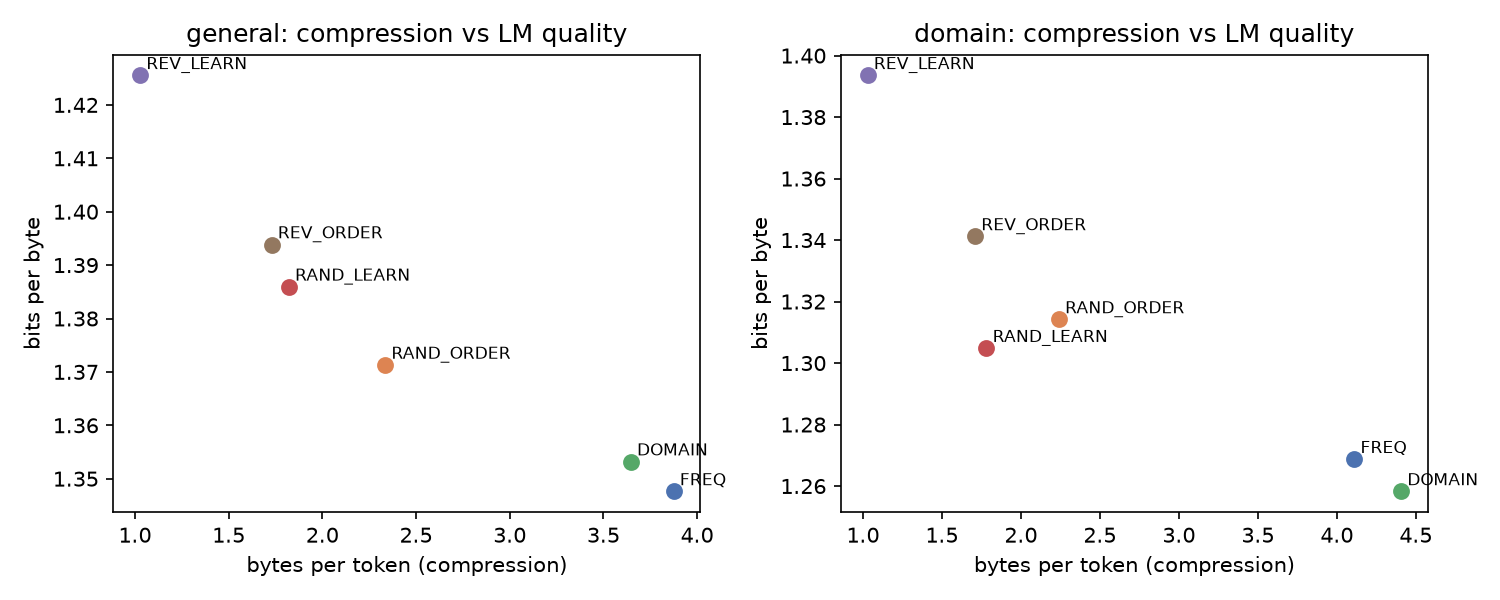
\includegraphics[width=0.95\linewidth]{figures/compression_vs_bpb.png}
    \caption{Compression predicts language-modeling quality. Each point is one tokenizer (mean of 2 seeds; labels use underscores, \eg \texttt{REV\_LEARN} is \revlearn). \figleft On general text, the rank of bytes-per-token matches the rank of \bpb exactly (Spearman $\rho=-1.0$, exact $p=0.003$). \figright On biomedical text the relation is nearly monotone ($\rho=-0.94$, $p=0.005$); \randlearn and \randorder swap places, and \domain overtakes \freq by compressing better.}
    \label{fig:compression}
\end{figure}

\para{Bytes per token rank-predicts \bpb.}
\Figref{fig:compression} plots \bpb against compression.
On general text, the ranks match exactly ($\rho=-1.0$, $n=6$).
On biomedical text, the relation is nearly perfect ($\rho=-0.94$).
The only swap is between \randlearn and \randorder, whose biomedical compression differs by 0.46 bytes per token while their \bpb differs by only 0.009.
Compression also explains \domain: it is the best compressor of biomedical text and the best biomedical model.

\para{R\'enyi efficiency does not.}
R\'enyi efficiency~\citep{zouhar2023tokenization} ranks the tokenizers differently.
\randorder has the \emph{highest} general R\'enyi efficiency (0.55, \tabref{tab:intrinsics}) but only the third-best \bpb.
Across the six tokenizers, R\'enyi efficiency correlates only weakly with \bpb ($\rho=-0.71$, $p=0.11$ on general text; $\rho=-0.49$, $p=0.33$ on biomedical text).
In our setting, plain compression is the better predictor.

\para{Why compression matters here.}
With a fixed 512-token window, a poor compressor sees much less text: about 530 bytes per window for \revlearn \versus about 2,000 bytes for \freq.
It also spends capacity on predicting pieces inside words.
The training curves in \figref{fig:train_curves} (\appref{app:extra}) are consistent with this.
The per-byte training loss of all tokenizers overlaps for most of training, and the gaps open late, as \freq and \domain keep improving.

\subsection{Merge order does not affect fine-tuned classification}
\label{sec:ft}

\begin{table}[t]
    \centering
    \caption{Fine-tuned accuracy (\%, mean $\pm$ sd over 4 runs) and relative change against \freq with 95\% paired-bootstrap CIs over test items. None of the 15 comparisons is significant (raw $p \ge 0.08$; Holm-adjusted $p = 1.0$). Best mean per task in \textbf{bold}. Macro-F1 gives the same picture (\tabref{tab:f1}).}
    \label{tab:finetune}
    \resizebox{\textwidth}{!}{%
    \begin{tabular}{@{}lcccccc@{}}
        \toprule
        & \multicolumn{2}{c}{\sst} & \multicolumn{2}{c}{\agnews} & \multicolumn{2}{c}{\pubmedrct (domain)} \\
        \cmidrule(lr){2-3} \cmidrule(lr){4-5} \cmidrule(lr){6-7}
        \textbf{Tokenizer} & Acc. & $\Delta$ [95\% CI] & Acc. & $\Delta$ [95\% CI] & Acc. & $\Delta$ [95\% CI] \\
        \midrule
        \freq      & 80.2 {\scriptsize $\pm$ 0.4} & --- & \textbf{89.3} {\scriptsize $\pm$ 0.4} & --- & 81.7 {\scriptsize $\pm$ 0.4} & --- \\
        \domain    & \textbf{81.5} {\scriptsize $\pm$ 0.4} & +1.57\% [$-$0.43, 3.66] & 88.9 {\scriptsize $\pm$ 0.4} & $-$0.48\% [$-$1.14, 0.20] & \textbf{81.8} {\scriptsize $\pm$ 0.3} & +0.07\% [$-$0.59, 0.75] \\
        \midrule
        \randlearn & 79.7 {\scriptsize $\pm$ 0.6} & $-$0.64\% [$-$3.34, 2.08] & 88.8 {\scriptsize $\pm$ 0.4} & $-$0.58\% [$-$1.41, 0.25] & 81.4 {\scriptsize $\pm$ 0.2} & $-$0.35\% [$-$1.24, 0.55] \\
        \revlearn  & 80.8 {\scriptsize $\pm$ 0.7} & +0.72\% [$-$1.72, 3.18] & 88.7 {\scriptsize $\pm$ 0.4} & $-$0.71\% [$-$1.57, 0.14] & 81.1 {\scriptsize $\pm$ 0.3} & $-$0.75\% [$-$1.69, 0.20] \\
        \midrule
        \randorder & 79.8 {\scriptsize $\pm$ 0.7} & $-$0.54\% [$-$2.96, 1.93] & 88.8 {\scriptsize $\pm$ 0.2} & $-$0.50\% [$-$1.29, 0.28] & 81.1 {\scriptsize $\pm$ 0.5} & $-$0.75\% [$-$1.60, 0.09] \\
        \revorder  & 80.0 {\scriptsize $\pm$ 0.9} & $-$0.21\% [$-$2.80, 2.53] & 88.9 {\scriptsize $\pm$ 0.4} & $-$0.46\% [$-$1.28, 0.37] & 81.1 {\scriptsize $\pm$ 0.2} & $-$0.81\% [$-$1.70, 0.07] \\
        \bottomrule
    \end{tabular}}
\end{table}


\begin{figure}[t]
    \centering
    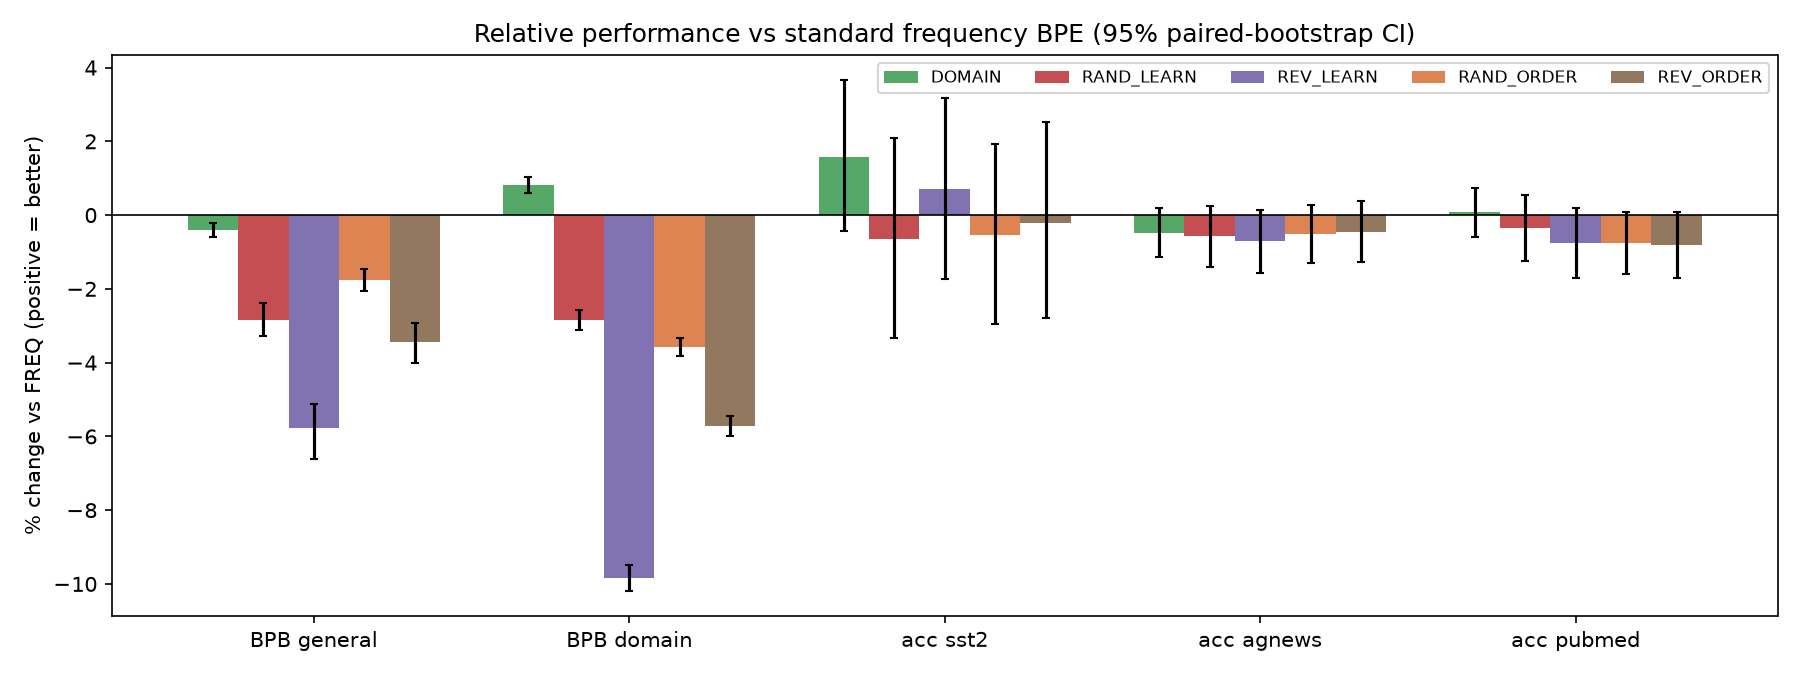
\includegraphics[width=0.95\linewidth]{figures/relative_vs_freq.png}
    \caption{Relative change against \freq with 95\% paired-bootstrap CIs; positive means better, so \bpb changes are sign-flipped. The language-modeling gaps (left two groups) are large and have tight intervals. The fine-tuning differences (right three groups) are small, and every interval covers zero.}
    \label{fig:relative}
\end{figure}

\para{All tokenizers reach the same accuracy.}
\Tabref{tab:finetune} and \figref{fig:relative} show that every tokenizer lands within $-0.8\%$ to $+1.6\%$ of \freq's accuracy.
None of the 15 comparisons is significant (raw $p \ge 0.08$, Holm-adjusted $p = 1.0$).
The confidence intervals are tight enough to be informative: they rule out effects larger than about 1.7\% on \agnews and \pubmedrct, and about 3.5\% on \sst.
On \pubmedrct, the four non-frequency tokenizers are all slightly below \freq ($-0.35\%$ to $-0.81\%$), but every interval includes zero.

\para{Even a near-character tokenizer is competitive.}
\revlearn, which needs 5.0 tokens per word, is within 1\% of \freq on every task.
This holds even on \agnews, where 23\% of \revlearn's test inputs are truncated at 256 tokens (\versus 0.1\% for \freq).
Its 5.8--9.8\% \bpb gap from pre-training simply does not carry over to these tasks.

\para{Domain weighting does not help the domain task.}
\domain improves \pubmedrct accuracy by only 0.07\%.
Its +1.6\% on \sst is the largest point gain in the table, but it is not significant ($p=0.13$, CI $[-0.43, 3.66]$).

\subsection{Robustness}
\label{sec:robustness}

\begin{table}[t]
    \centering
    \caption{Robustness to the random draw. A second draw (\textsc{-t1}) of each random tokenizer, trained with pre-training seed 0, gives effects of the same size as the first draw. $\Delta$ is relative to \freq seed 0. Accuracy (\%) is the mean of 2 fine-tuning seeds on the seed-0 model; differences between draws are within 0.7 points on every task.}
    \label{tab:robustness}
    \resizebox{\textwidth}{!}{%
    \begin{tabular}{@{}lcccccc@{}}
        \toprule
        \textbf{Tokenizer} & \textbf{Bytes/token} & \textbf{General $\Delta$\bpb} & \textbf{Domain $\Delta$\bpb} & \textbf{\sst} & \textbf{\agnews} & \textbf{\pubmedrct} \\
        \midrule
        \randorder          & 2.34 & +1.7\% & +3.7\% & 80.1 & 88.8 & 81.1 \\
        \randorder\textsc{-t1} & 2.19 & +2.5\% & +2.3\% & 79.5 & 88.6 & 81.1 \\
        \midrule
        \randlearn          & 1.82 & +3.0\% & +3.4\% & 79.6 & 88.5 & 81.4 \\
        \randlearn\textsc{-t1} & 1.76 & +2.7\% & +5.3\% & 79.0 & 89.0 & 81.5 \\
        \bottomrule
    \end{tabular}}
\end{table}


\para{Random draw.}
\Tabref{tab:robustness} shows that a second random draw of each random tokenizer gives effects of the same size: +1.7--3.0\% general \bpb across all four random tokenizers, and accuracy within 0.7 points of the first draw.
Our conclusions do not depend on the particular permutation.

\para{Seeds.}
The pre-training seed standard deviation of \bpb ($\le 0.016$) is much smaller than the gaps between \freq and the four non-frequency orders ($\ge 0.024$), and the fine-tuning standard deviation ($\le 0.9$ points) is similar to the between-tokenizer differences.

\para{Compute does not compensate.}
Because we hold text fixed, poor compressors get more tokens and more gradient steps: 1.7--3.8$\times$ the compute of \freq (\tabref{tab:compute}, \appref{app:extra}).
\revlearn takes 5,939 steps, while \freq takes 1,555.
\freq is still best on general text.
An equal-compute comparison would therefore favor \freq even more.

\subsection{Hypothesis verdicts}
\label{sec:verdicts}

\begin{table}[t]
    \centering
    \caption{The four hypotheses we set out to test and their verdicts. The qualitative ordering largely holds for \bpb, but the hypothesized effect sizes are too large, and none of the effects reaches fine-tuned accuracy.}
    \label{tab:hypotheses}
    \small
    \begin{tabular}{@{}p{4.4cm}p{6.2cm}l@{}}
        \toprule
        \textbf{Hypothesis} & \textbf{Observed} & \textbf{Verdict} \\
        \midrule
        H1: \freq beats alternatives by 3--8\% on general tasks & \bpb: +1.8--5.8\%; accuracy: $\le$1.6\%, n.s. & Partly (\bpb only) \\
        H2: \domain beats \freq by 5--12\% on its domain & \bpb: 0.8\%; accuracy: 0.07\%, n.s. & Not supported \\
        H3: Random order is only 2--5\% worse & \bpb: +1.8--3.6\%; accuracy: $\approx$0.5\%, n.s. & Roughly (\bpb) \\
        H4: Reverse-frequency degrades most (10--20\%) & Worst for \bpb (+5.8\% / +9.8\%); not for accuracy & Direction only \\
        \bottomrule
    \end{tabular}
\end{table}


\Tabref{tab:hypotheses} summarizes our initial hypotheses.
The qualitative picture largely holds for \bpb: \freq wins on general text, random orders lose a few percent, and reverse-frequency is worst.
However, the hypothesized effect sizes are too large.
Reverse frequency loses 5.8--9.8\% rather than 10--20\%, and domain weighting gains 0.8\% rather than 5--12\%.
None of the effects reaches fine-tuned accuracy.
